\documentclass{article}
\usepackage[utf8]{inputenc}
\usepackage{geometry}
\geometry{
 a4paper,
 total={170mm,257mm},
 left=20mm,
 top=20mm,
}
\usepackage{graphicx}
\usepackage{titling}
\usepackage{listings}
\usepackage[hyphens]{url} 
\usepackage{listings}
\usepackage{xcolor}

\definecolor{codegreen}{rgb}{0,0.6,0}
\definecolor{codegray}{rgb}{0.5,0.5,0.5}
\definecolor{codepurple}{rgb}{0.58,0,0.82}
\definecolor{backcolour}{rgb}{0.95,0.95,0.92}

\lstdefinestyle{mystyle}{
    backgroundcolor=\color{backcolour},   
    commentstyle=\color{codegreen},
    keywordstyle=\color{magenta},
    numberstyle=\tiny\color{codegray},
    stringstyle=\color{codepurple},
    basicstyle=\ttfamily\footnotesize,
    breakatwhitespace=false,         
    breaklines=true,                 
    captionpos=b,                    
    keepspaces=true,                 
    numbers=left,                    
    numbersep=5pt,                  
    showspaces=false,                
    showstringspaces=false,
    showtabs=false,                  
    tabsize=2
}

\lstset{
    language=Python,
    frame=single,
    backgroundcolor=\color{lightgray},
    basicstyle=\ttfamily\footnotesize,
    keywordstyle=\color{blue},
    commentstyle=\color{green!60!black},
    stringstyle=\color{red},
    showstringspaces=false
}

\usepackage{hyperref}
\usepackage{glossaries} % Ajout du package pour le glossaire

\title{ChatBot Langchain pour l'UQAC}
\author{Mathis A., Ryan C., Samuel M.}
\date{\today}
 
\usepackage{hyperref}
\usepackage{fancyhdr}
\fancypagestyle{plain}{%  the preset of fancyhdr 
    \fancyhf{} % clear all header and footer fields
    \fancyfoot[L]{\thedate}
    \fancyfoot[R]{\includegraphics[width=2cm]{UQAC_Logo.png}} % Logo et numéro de page en bas à droite
    \fancyhead[L]{ChatBot Langchain pour l’UQAC}
    \fancyhead[R]{\theauthor}
}

% Appliquer le même style à toutes les pages
\pagestyle{fancy}
    \fancyhead[L]{ChatBot Langchain pour l’UQAC}
    \fancyhead[R]{\theauthor}
\fancyfoot[L]{\thedate}
\fancyfoot[R]{\includegraphics[width=2cm]{UQAC_Logo.png}} % Logo et numéro de page en bas à droite

\makeatletter
\def\@maketitle{%
  \newpage
  \null
  \vskip 1em%
  \begin{center}%
  \let \footnote \thanks
    {\LARGE \@title \par}%
    \vskip 1em%
    %{\large \@date}%
  \end{center}%
  \par
  \vskip 1em}
\makeatother

\usepackage{lipsum}  
\usepackage{cmbright}

\begin{document}

\maketitle
\noindent\begin{tabular}{@{}ll}
    Réalisé par :\\
        & Mathis Aulagnier - AULM12040200 \\
        & Ryan Collobert - COLR28120200 \\
        & Samuel Madrigal - MADS23060200 \\
        \\
    Cours :  &  8INF974 – ATELIER PRATIQUE EN INTELLIGENCE ARTIFICIELLE II \\
\end{tabular}

\section{Introduction}

\subsection{État des lieux}
\quad L'Université du Québec à Chicoutimi (UQAC) regroupe plus de 6500 étudiants répartis dans plus de 200 programmes d'études. Pour assurer sa gestion administrative, l'université dispose d'un manuel de gestion qui regroupe l'ensemble des règlements, politiques et procédures. Face au volume croissant de ce manuel, les employés rencontrent des difficultés pour retrouver rapidement l'information nécessaire.\\

Dans le cadre du cours 8INF974 - Atelier pratique en intelligence artificielle II, notre équipe de trois étudiants a été mandatée pour développer une preuve de concept d'un chatbot. Ce projet s'inscrit dans une démarche d'innovation, exploitant les récentes avancées en traitement du langage naturel (NLP) et en apprentissage automatique (ML).

\subsection{Objectifs}
\quad Notre projet vise à créer un assistant conversationnel capable de répondre efficacement aux questions des employés concernant le manuel de gestion. Pour atteindre cet objectif, nous explorons la mise en œuvre de chatbots avec LangChain, intégrons l'intelligence artificielle dans une application web, et approfondissons nos connaissances dans le développement d'IA.\\
\\
Notre solution s'appuie sur la technique RAG (Retrieval Augmented Generation), qui combine deux étapes clés : 
\begin{itemize} 
    \item Le Retrieval (Récupération) : recherche des informations pertinentes dans une base de données en fonction de la question posée 
    \item L'Augmented Generation (Génération Augmentée) : utilisation des informations récupérées pour enrichir le contexte et générer une réponse précise via un modèle de langage 
\end{itemize}
En combinant ces deux étapes, le RAG peut produire des réponses plus précises et contextuellement appropriées.\\

Pour des raisons de confidentialité et de coûts, notre solution utilise un modèle de langage hébergé localement plutôt qu'un service cloud.

\clearpage

\section{Scraping des Pages Web}

Notre approche de scraping a évolué en trois phases distinctes pour optimiser la qualité des données extraites :

\begin{enumerate}
    \item \textbf{Scraping Initial} \\
    La première approche a été réalisée avec un script Python basique effectuant du drill-down sur le site. Cette méthode a révélé des limitations importantes dues à la structure répétitive des pages (table des matières et sommaire redondants).
    
    \item \textbf{Optimisation du Script} \\
    Amélioration du script pour :
    \begin{itemize}
        \item Supporter l'extraction des fichiers PDF
        \item Cibler spécifiquement les balises "Article"
        \item Filtrer les éléments HTML indésirables
    \end{itemize}
    
    \item \textbf{Solution Finale avec Crawl4AI} \\
    La découverte du dépôt \texttt{Crawl4AI} sur GitHub (\href{https://github.com/unclecode/crawl4ai}{https://github.com/unclecode/crawl4ai}) a été notre choix final pour le scrapping. Cette bibliothèque, spécialement conçue pour l'extraction de données destinées aux modèles de langage, offre plusieurs avantages cruciaux :
    
    \begin{itemize}
        \item \textbf{AsyncWebCrawler} : Cette bibliothèque facilite le traitement parallèle des requêtes, ce qui diminue considérablement le temps nécessaire pour extraire les données. Sa capacité à gérer les opérations de manière asynchrone est particulièrement utile pour traiter le grand nombre de pages de notre manuel de gestion. Cependant, nous avons dû changer notre adresse IP à plusieurs reprises car le site de l'UQAC nous a bannis en raison de l'envoi soudain d'un trop grand nombre de requêtes.
        
        \item \textbf{DefaultMarkdownGenerator} : Ce composant assure une conversion fidèle du contenu HTML/PDF en Markdown, préservant la structure des documents tout en les rendant plus accessibles pour notre chaîne de traitement RAG.
        
        \item \textbf{Le nettoyage du contenu} est optimisé grâce aux filtres préconfigurés de Crawl4AI. Notre script \texttt{getArticle.py} utilise notamment le \texttt{PruningContentFilter} avec un seuil de 0.4, permettant de:
        \begin{itemize}
            \item Isoler le contenu pertinent dans les balises "article"
            \item Supprimer les éléments de navigation redondants
            \item Éliminer les publicités et contenus non pertinents
        \end{itemize}
    \end{itemize}
\end{enumerate}

Finalement, notre script \textit{getURL.py} utilise le sitemap.xml du site pour cartographier en profondeur le site. Le sitemap nous a notamment permis d'identifier plus de \textbf{293} pages pertinentes à traiter.

\clearpage

\section{Conception de notre RAG}

\subsection{Contexte et Objectifs}
\quad La mise en place d'un système RAG (Retrieval-Augmented Generation) nécessite une recherche approfondie sur les méthodes de construction et les optimisations possibles. Notre démarche a débuté par l'identification des formats de données les plus adaptés aux modèles de langage. Le format Markdown s'est imposé naturellement, offrant une structure claire tout en restant simple à manipuler. Cette décision a guidé notre choix d'utiliser \texttt{crawl4AI} pour l'extraction des données, nous permettant ainsi d'obtenir directement un format optimal pour la suite du traitement.
    
\subsection{Comparaison des Architectures de Chatbots}
    \subsubsection{Le Chatbot Traditionnel}
    \quad Le chatbot basé sur un graphe représente l'approche la plus conventionnelle. Il fonctionne avec un ensemble prédéfini de questions et réponses stockées dans une base de données relationnelle. Bien que cette méthode garantisse des réponses rapides et précises pour les cas anticipés, elle souffre d'un manque crucial de flexibilité. L'impossibilité de traiter des questions non prévues limite considérablement son utilité dans des contextes dynamiques.\\
    \\
    Voici, le schéma présentant l'architecture du chatbot traditionnel : 
    \begin{figure}[ht]
        \centering
        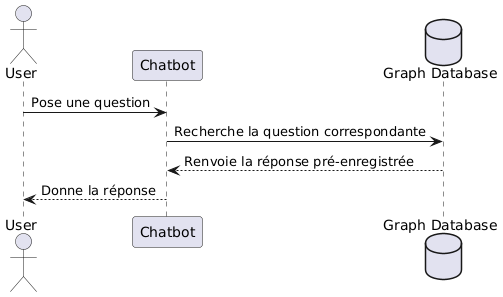
\includegraphics[width=0.5\textwidth]{chatbot_graphe.png}
        \caption{Architecture d’un chatbot basé sur un graphe}
    \end{figure}
    
    \subsubsection{L'Évolution vers les LLM}
    \quad L'introduction des modèles de langage (LLM) a marqué une évolution majeure pour les chatbots. Ces systèmes génèrent des réponses en s'appuyant sur leur compréhension du langage naturel, acquise lors de leur entraînement. Bien que plus flexibles que leurs prédécesseurs, ils présentent une limitation importante : l'absence de connexion à des sources d'information externes actualisées. Cette caractéristique peut conduire à des réponses imprécises ou obsolètes, particulièrement dans des domaines spécialisés.\\
    \\
    Voici, le schéma présentant l'architecture du chatbot connecté à un LLM : 
    \begin{figure}[ht]
        \centering
        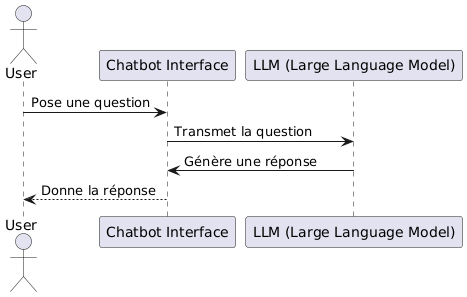
\includegraphics[width=0.5\textwidth]{LLM.png}
        \caption{Architecture d’un chatbot basé sur un LLM}
    \end{figure}
    
    \subsubsection{L'Innovation RAG}
    \quad Le système RAG représente une synthèse innovante, combinant les avantages des deux approches précédentes. En associant la puissance générative d'un LLM à une base de connaissances externe, il permet de produire des réponses à la fois contextuelles et factuellement précises. Cette architecture permet une mise à jour continue des connaissances sans nécessiter de réentraînement du modèle.\\
    \\
    Voici, le schéma présentant l'architecture d'un RAG :
    \begin{figure}[ht]
        \centering
        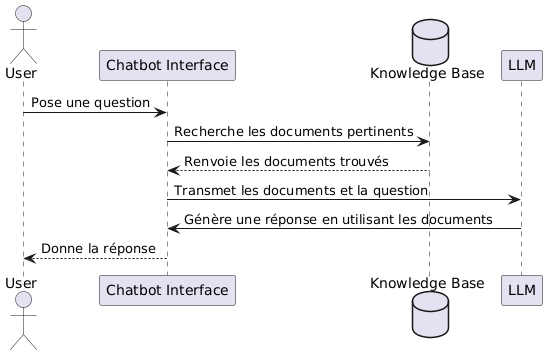
\includegraphics[width=0.5\textwidth]{RAG.png}
        \caption{Architecture d’un chatbot basé sur un RAG}
    \end{figure}

\subsection{Système de Recherche Intelligent}
    \subsubsection{Défis de la Recherche Documentaire}
    \quad La recherche efficace dans une base documentaire pose un défi majeur. Une approche par mots-clés simples s'avère souvent insuffisante, produisant trop de résultats sans garantie de pertinence contextuelle. Notre solution repose sur l'utilisation d'embeddings, permettant une compréhension plus profonde du contexte des requêtes.
    
    \subsubsection{Vectorisation Sémantique}
    \quad Notre système transforme aussi bien les questions que les documents en vecteurs numériques grâce au modèle Llama3. Ces vecteurs de dimension 4096 capturent les nuances sémantiques du texte, permettant des comparaisons précises basées sur la similarité conceptuelle plutôt que sur la simple correspondance de mots.

\subsection{Innovations Techniques}
    \subsubsection{Traitement et Segmentation des Données}
    \quad La gestion efficace des données extraites constitue un défi majeur dans notre architecture RAG. Les documents Markdown, bien que correctement structurés, sont souvent trop volumineux pour être traités directement par les modèles de langage. Pour résoudre ce problème, nous avons implémenté un système de découpage intelligent utilisant \texttt{MarkdownTextSplitter} de Langchain.\\
    
    Cette approche permet de diviser les documents en segments (chunks) tout en préservant leur cohérence sémantique. Le système maintient un recouvrement (overlap) entre les segments consécutifs, garantissant ainsi la conservation du contexte global. Cette méthode s'est révélée particulièrement efficace pour respecter les contraintes de tokens des modèles tout en préservant l'intégrité de l'information.
    
    \subsubsection{Enrichissement par Métadonnées}
    Chaque chunk généré est enrichi avec un ensemble de métadonnées cruciales :
    \begin{itemize}
        \item L'URL source du document original
        \item La position relative dans le document
        \item Les informations contextuelles essentielles
    \end{itemize}
    Cette structuration permet non seulement la traçabilité des informations mais facilite également la reconstitution du contexte complet lorsque nécessaire.
    
    \subsubsection{Architecture de Stockage}
    \quad Le choix de Chroma DB comme base de données vectorielle représente un élément clé de notre architecture. Cette solution offre des capacités d'indexation et de recherche optimisées pour les vecteurs de haute dimension, garantissant des temps de réponse rapides même sur de grands volumes de données. Le processus complet suit une séquence logique :
    \begin{enumerate}
        \item Prétraitement et segmentation des documents
        \item Vectorisation des chunks via Llama3
        \item Stockage structuré dans Chroma DB
    \end{enumerate}
    
    \subsubsection{Gestion Contextuelle}
    \quad Notre système maintient la cohérence des informations grâce à une gestion sophistiquée des métadonnées. Chaque fragment de texte conserve ses liens avec le document source et son contexte d'origine, permettant une reconstitution fidèle de l'information complète lorsque nécessaire.
    
    \subsubsection{Optimisation des Performances}
    \quad L'architecture a été conçue pour équilibrer précision et rapidité. Le système de chunking intelligent, combiné à l'indexation vectorielle, permet de maintenir des temps de réponse optimaux tout en garantissant la pertinence des résultats. La taille des chunks a été choisi afin d'avoir assez d'information et assezcours pour eviter des erreur de token overflow .

\clearpage

\section{Implémentation du Chatbot}
\subsection{Architecture du RAG}
\begin{figure}[ht]
    \centering
    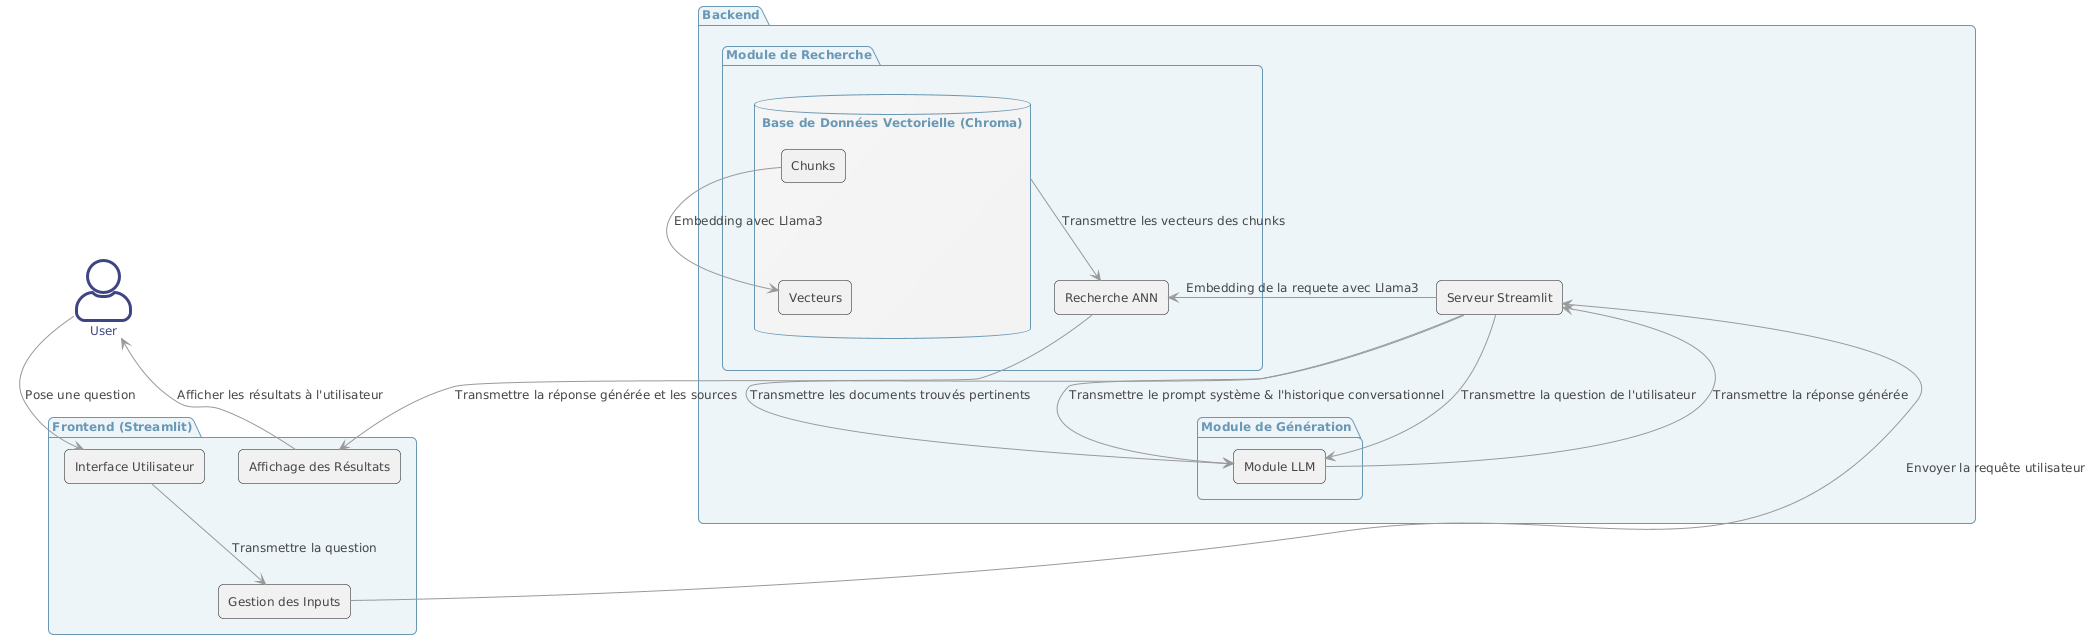
\includegraphics[width=\textwidth]{NotreRAG2.png}
    \caption{Architecture d’un chatbot basé sur un RAG}
\end{figure}

\subsection{Choix du Modèle Local}
    \subsubsection{GPT 3.5 et GPT-2}
    \quad Notre objectif était d'utiliser un modèle fonctionnant en local, ce qui impliquait de choisir des modèles de petite taille. Nous avons d'abord testé GPT-3.5, mais celui-ci présentait une limitation à 500 tokens, ce qui le rendait quasi inutilisable dans le cadre de ce projet. Nous sommes ensuite passés à GPT-2.0, mais celui-ci posait également des problèmes, notamment parce qu'il avait été principalement entraîné en anglais. Or, l'UQAC fournit les fichiers de documentation en français, ce qui entraînait des difficultés de compréhension et de génération.
    
    \subsubsection{Mistral}
    Nous nous sommes alors tournés vers des modèles spécifiquement développés pour le traitement du français ou, au moins, capables de le comprendre. Cependant, ces modèles étaient dépassés en termes de performances, car ils ne faisaient plus partie des modèles \textit{state-of-the-art} (ex : FlauBERT, un dérivé de BERT). Nous avons donc ensuite opté pour Mistral, qui possédait plus de tokens que GPT-3.5 et une meilleure compréhension du français que GPT-2.0 (bien que limitée).
    
    \subsubsection{DeepSeek 8B}
    Avec l'apparition de DeepSeek, nous avons migré vers ce LLM, car il permettait d'obtenir des réponses de meilleure qualité et en français. Cependant, nous avons encore rencontré des problèmes : DeepSeek ignorait parfois les instructions et générait des réponses aléatoires.
    
    \subsubsection{Choix Final : LLaMA 3.0}
    Finalement, après plusieurs tests comparatifs, nous avons choisi LLaMA 3.0 pour les raisons suivantes :
    \begin{enumerate}
        \item Il est également utilisé pour effectuer les embeddings (voir l'architecture RAG), donc il n'y a que un seul model qui est chargé sur la RAM.
        \item Il fournit les réponses les plus pertinentes.
        \item Il possède un nombre suffisant de tokens (4k) pour permettre un système de mémoire.
    \end{enumerate}

\subsection{Interface Utilisateur}
\quad Pour l'Interface Utilisateur, nous avons utilisé Streamlit, car nous codons en Python. Cette solution permet de générer une interface web sans changer de langage, assurant ainsi une cohérence de langage dans le projet.\\

Notre objectif initial était de concevoir une interface visuellement proche des pages de l'UQAC. Cependant, nous avons rencontré plusieurs difficultés, notamment avec le thème par défaut de Streamlit, qui reste sombre à moins que l'utilisateur ne le modifie lui-même, ainsi qu'avec le header de Streamlit, qui masque notre propre en-tête, cachant des informations que nous souhaiton donner a l'utilisateur.\\

Face à ces contraintes, nous avons finalement choisi de conserver une interface Streamlit simple, sans ajout de CSS personnalisé pour que l'utilisateur ne perdes pas d'information et qu'il n'ai "rien a faire" d'autre que de poser des questions au chatbot.\\
\\
(image exemple page uqac, notre interface style uqac et interface finale ici)

\clearpage

\section{Résultats}
\subsection{Performance du Système}
\quad L'application finale utilise LLaMA 3 (8B paramètres, nécessitant 8GB de RAM) ainsi qu'une base de données Chroma DB (occupant 1GB de RAM). Les autres composants de l'application ont un impact négligeable sur les performances. Ainsi, lors de son exécution, l'application consomme un total d'environ 9GB de RAM.
\begin{figure}[ht]
    \centering
    \includegraphics[width=\textwidth]{perfs.png}
    \caption{Performances de l'application}
\end{figure}
\subsection{Exemples de Conversations}
faire a la fin ducoup...
\clearpage

\section{Défis et Apprentissages}
\subsection{Problèmes Rencontrés}

Au cours de ce projet, nous avons été confrontés à plusieurs défis techniques et conceptuels :

\begin{itemize}
    \item \textbf{Problèmes de scraping :} La première version du scraping ne récupérait pas les bons fichiers, ce qui a nécessité des ajustements. De plus, notre version finale a entraîné un bannissement temporaire du site de l'UQAC en raison d'un trop grand nombre de requêtes.
    \item \textbf{Problèmes d'affichage du chatbot :} L'intégration du chatbot dans une interface inspirée du style de l'UQAC a posé des difficultés, notamment avec le thème de Streamlit, qui restait sombre par défaut ainsi que le header de Streamlit, qui masquait notre propre en-tête.
    \item \textbf{Réponses en anglais du LLM :} Certains modèles de langage répondaient en anglais alors que nous avions besoin de réponses en français.
    \item \textbf{Gestion des flux de réponse :} Notre approche reposait sur deux flux de sortie : les réponses aux questions et les sources associées. Cependant, cela entraînait un problème d'affichage, l'une des deux réponses n'apparaissant pas toujours correctement.
    \item \textbf{Coupures dans les réponses :} Certaines réponses étaient tronquées en raison de la limite de tokens imposée par certains modèles de langage.
    \item \textbf{Gestion de la mémoire :} La limite du nombre de tokens nous empêchait de conserver l'intégralité de la conversation en mémoire.
    \item \textbf{Besoins en contexte des LLMs :} Certains modèles nécessitaient plus de contexte que d'autres pour fournir des réponses pertinentes, ce qui nous a poussés à ajuster la manière dont nous leur fournissions les données.
\end{itemize}

\subsection{Solutions Apportées}

\begin{itemize}
    \item \textbf{Scraping :} 
    \begin{itemize}
        \item \textbf{Version 1} : Remplacement du scraping initial par l'utilisation de \texttt{crwl4ai}.
        \item \textbf{Version 2} : Changement d'adresse IP à chaque bannissement pour contourner les restrictions du site de l'UQAC.
    \end{itemize}
    
    \item \textbf{Interface :} Mise en pause temporaire du développement de l'interface pour prioriser d'autres aspects critiques du projet.
    
    \item \textbf{Gestion des réponses en anglais :} 
    \begin{itemize}
        \item \textbf{Changement de LLM} : Passage de GPT-3.5 à DeepSeek (qui répond nativement en francais), puis à LLaMA 3 (méthode hybride).
        \item \textbf{Méthode hybride pour LLaMA 3} :  
        \begin{enumerate}
            \item Première requête pour obtenir la réponse avec les sources (générées en anglais).
            \item Seconde requête pour traduire la réponse en français.
        \end{enumerate}
    \end{itemize}

    \item \textbf{Gestion du multi-flux :}  
    Le code suivant permet de récupérer simultanément la réponse et ses sources :
    
    \begin{verbatim}
    qa_chain = ConversationalRetrievalChain.from_llm(
        llm=llm,
        retriever=retriever,
        memory=memory,
        return_source_documents=True,
        output_key="answer"
    )
    \end{verbatim}

    Ainsi, la réponse du LLM est récupérée via \texttt{output\_key="answer"} et les sources via \texttt{return\_source\_documents=True}, ce qui permet de traiter les deux flux simultanément.

    \item \textbf{Limite de tokens :}  
    Passage de GPT-3.5 (capacité de 500 tokens) à DeepSeek (capacité de 8000 tokens), puis à LLaMA 3 (capacité de 4000 tokens). Cette dernière limitation est compensée par une gestion optimisée de la mémoire.

    \item \textbf{Gestion de la mémoire :}  
    Deux approches ont été testées :
    \begin{itemize}
        \item \textbf{Première approche (non retenue)} : Une mémoire à une durée limitée, où le chatbot ne se souvenait que de la dernière question et de la dernière réponse avant la question actuelle.
        \item \textbf{Deuxième approche (retenue)} : Génération dynamique d’un résumé des échanges précédents, fourni au LLM à chaque nouvelle requête. Cette méthode permet une gestion efficace de l’espace mémoire tout en assurant une continuité des interactions sur toute la durée d'utilisation.
    \end{itemize}

    \item \textbf{Optimisation du contexte :}  
    \begin{itemize}
        \item Passage de 3 à 10 chunks pour élargir le contexte fourni au LLM.
        \item Remplacement de \textbf{kNN} par \textbf{aNN} :
        \begin{itemize}
            \item Le kNN fournit des résultats déterministe qui sont normalement plus précis.
            \item Le aNN est plus rapide et, combiné avec un plus grand nombre de chunks, garantit une réponse pertinente. Dans l'éventualité où ce n'est pas le cas, il est possible de reposer la question afin d'essayer de trouver de meilleurs chunks, ce qui n'est pas réalisable avec un kNN.
        \end{itemize}
    \end{itemize}
\end{itemize}


\subsection{Améliorations Possibles}
\begin{itemize}
    \item \textbf{Optimisation du scraping :}  
    Trouver un moyen de limiter la vitesse du scraping afin d'éviter le bannissement du site de l'UQAC, ou automatiser un changement d'IP dès qu'un bannissement est détecté.
    
    \item \textbf{Refonte du frontend :}  
    Abandonner Streamlit pour l'interface utilisateur et développer une page web en utilisant le même langage que celui des sites de l'UQAC. Cela permettrait une séparation plus nette entre le frontend et le backend. Actuellement, avec Streamlit, ces deux parties sont imbriquées dans le même fichier, ce qui "complique" l'architecture du projet pour d'eventuelles évolutions (comme l'implémentation du chatbot sur le site de l'UQAC).
    
    \item \textbf{Gestion améliorée de la mémoire et du contexte :}  
    Utiliser un package combinant Streamlit et LangChain afin d'optimiser la gestion de la mémoire et du contexte de conversation de manière plus efficace qu'actuellement.
\end{itemize}


\clearpage

\section{Conclusion}
\subsection{Bilan du Projet}
faire a la fin...
\subsection{Perspectives}
passer sur des LLMs plus puissants comme chatGPT qui permet actuellemet de chercher le web et de repondre a nos questions directement.

\end{document}